\documentclass[msthesis.tex]{subfiles}

\begin{document}
\chapter{Results}
In this section, the quanutitative and visualization results from the methods presented in the chapter \ref{chap:methods} will be presented. 
\section{Preprocessing Visualization}

In the process of generating the connectome \autoref{subsec:connectome_generation}) visual inspection was required to understand and investigate the properties of different types of images produced. 

In order to get an inspection of the working of the pipeline, the following results were obtained by visually inspecting the results. The 5TT image obtained was 4D and could not be easily displayed in 3D. Here it is displayed according to the grayscale mapping in 3D, it was observed that the 5TT images did not contain any errorneous labels. In this 4D image, each volume represents the corresponding tissue densities of WM, GM and CSF. The 4D image is then visualized as an RGB image with each volume getting its specific color (Fig. \ref{fig:preproc}(b)). With the help of the RGB image the alignment of the fODFs seemed sensible. 

Further, the one million fibers tractography was obtained with correspondence to the color coding of the fibers that run along the x.y and z axes respectively. The nodes of the connectome were then represented by the center of mass in the parcellated regions, the intensity of the image does not represent signal intensity but different parcels. 
\begin{figure}
    \centering
    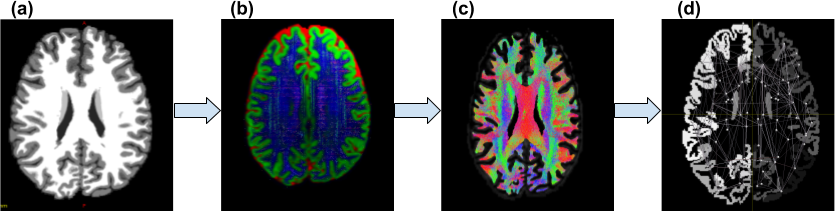
\includegraphics[width=\textwidth]{images/Preprocessing_pipeline.png}
    %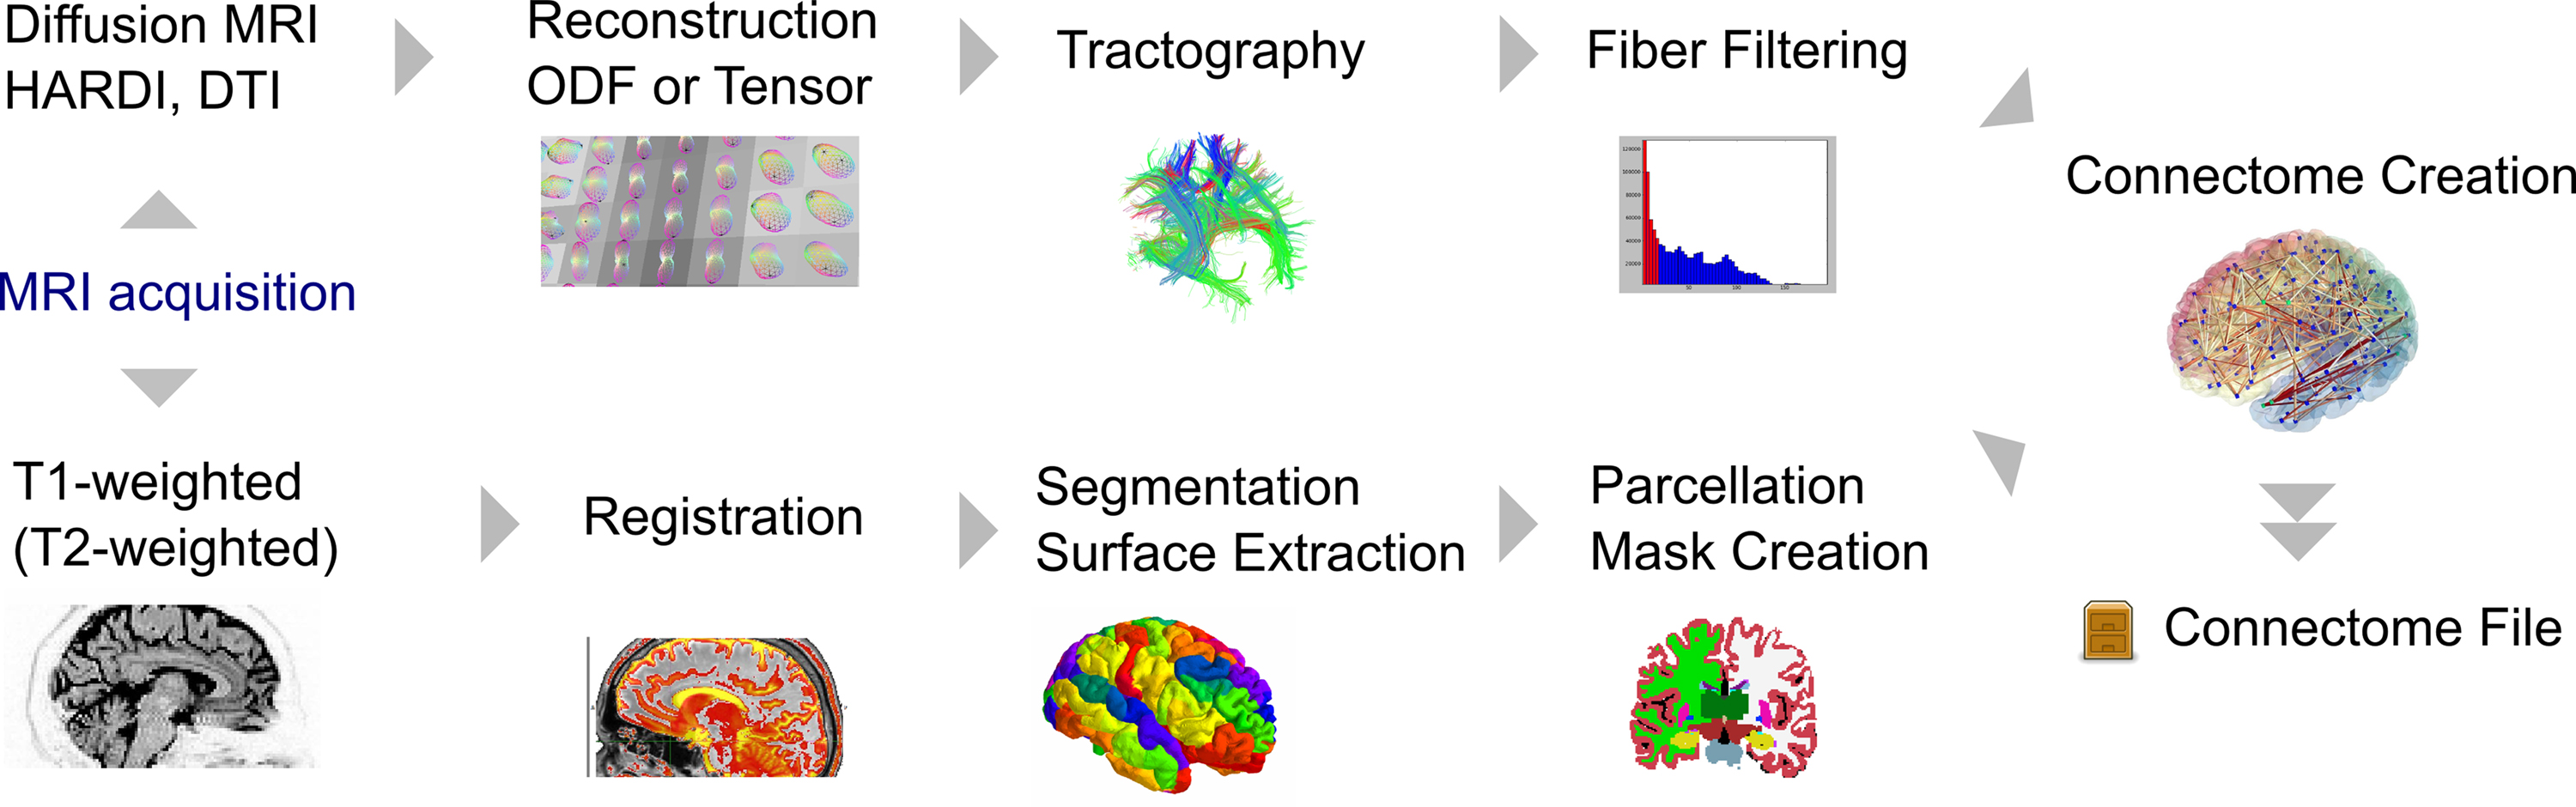
\includegraphics[width=\textwidth]{images/connectome_creation_workflow.png}
    %\cite{gerhard2011connectome}
    \caption{Visualization of pipeline used to create a connectome for each subject (a) Five tissue segmented image visualized in grayscale. (b) A slice of a 4D image mapped in 3D using RGB encoding tissue densities, CSF as red, GM as green and WM as blue. (c) Fiber tractography of one million fibers produced using probabilistic tractography overlaid on an axial slice of the brain. (d) The nodes of the connectome representing ROIs overlaid on an axial slice}
    \label{fig:preproc}
\end{figure}

\section{Connectome Visualization}

The individual connectome can be visualized using the connectivity matrices

In the chord plot represented in \autoref{fig:connectome_num_streamlines} the selection of the cortical region isthmus cingulate in the right hemisphere shows its prominent connections to the cortical regions inferior parietal, superior frontal, superior temporal in the left hemisphere as well as connections to the subcortical regions Hippocampus, Putamen and thalamus proper in the right hemisphere. Another weak connection is in right hemisphere cortical region fusiform. The interactive visualization helped determine the connections between brain regions. 
\label{sec:connectome_generation}
\begin{figure}
    \centering
    %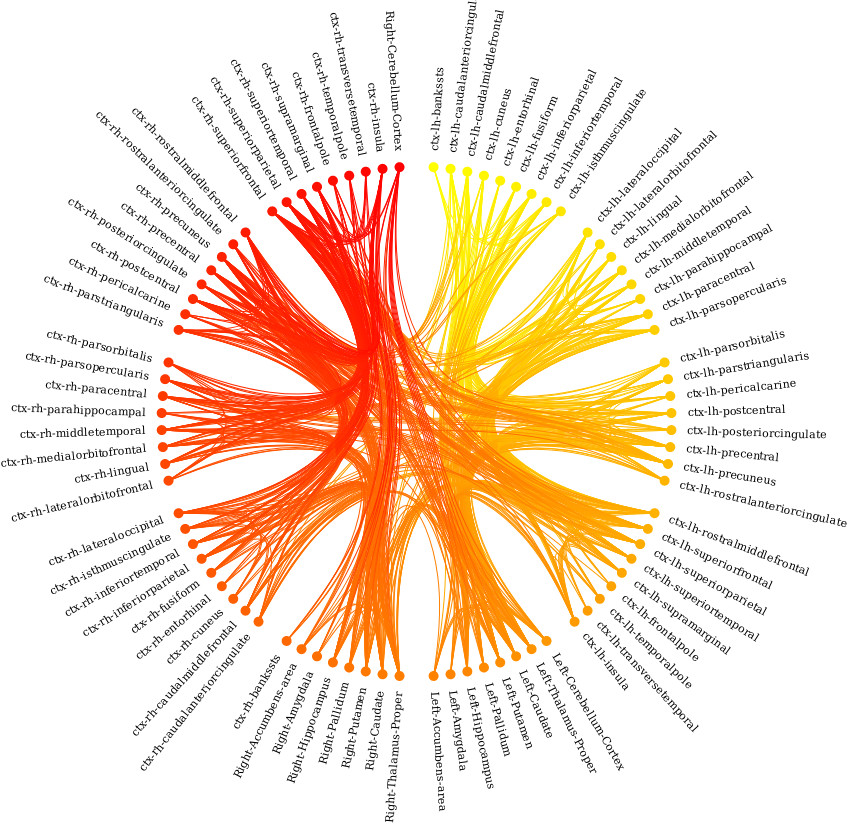
\includegraphics[width=\textwidth]{images/brain-data-viewer_2.png}
    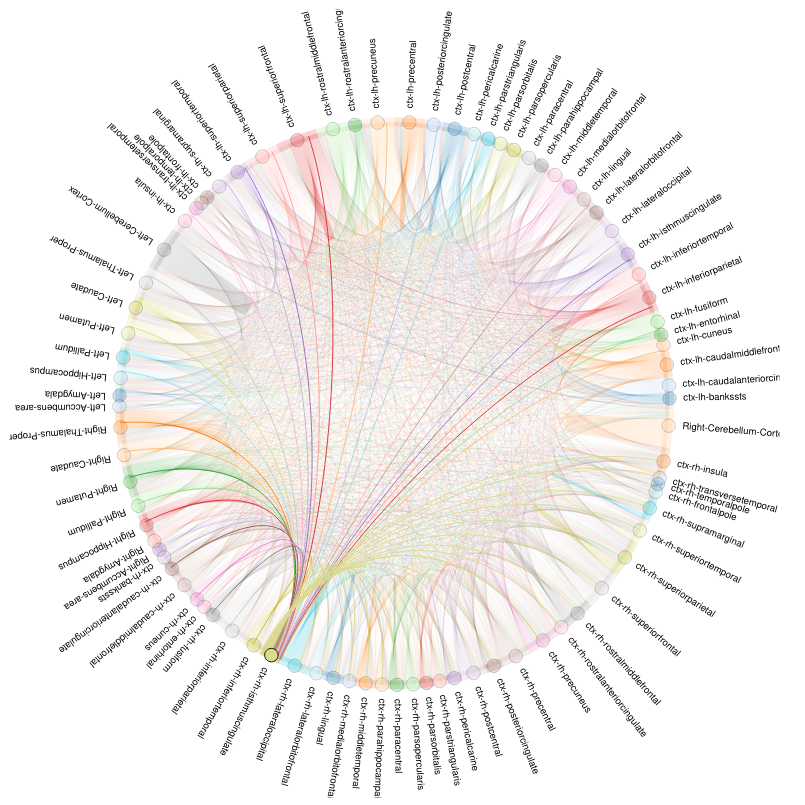
\includegraphics[width=\textwidth]{images/bokeh_plot_allsubjects.png}
    \caption{A choord plot representing the group averaged connectome for all subjects. The arcs(edges) represent the number of streamlines between any two ROIS. The ROIs are represented as the nodes in the diagram at the end of the circle and are lablled according to the Desikan Killiany Atlas. Chord diagram using the tool library Edge bundling also takes place. In this interactive visualization the cortical region isthmusvingulate is selected as the source node and the all the edges convergent on this node are colored according to the terminal node. The number of edges between any two nodes is the number of streamlines, multiple edges get bundled here.}
    \label{fig:connectome_num_streamlines}
\end{figure}

\section{Feature Analysis}
\subsection{Differences in the type of feature}
\iffalse
To be included in the methods chapter: first the different types of features were considered separately. Using Standard scalar the features were standardized by removing the mean and scaling to unit variance. After scaling the feature value for each subject is represented by a z statistic. Now once the type of feature (such as mean FA) is selected, then the mean z statistic was taken. Each type of feature has the upper triangular features excluding the diagonal features. So for each type of feature there are 3570-84 features.  
\fi
The distribution for the number of streamlines for males and females in the training data are both non-overlapping and well-normally distributed. This could contribute towards the good performance of classifiers when training on the basis of number of streamlines. 
\begin{figure}
    \centering
    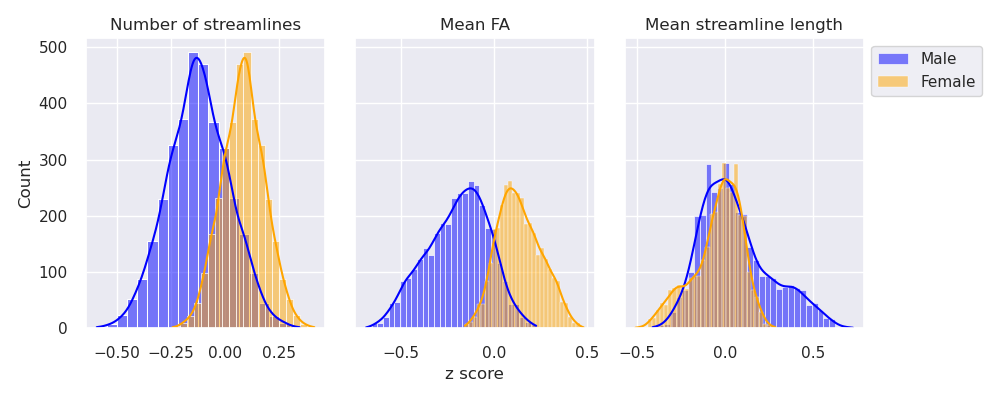
\includegraphics[width=\textwidth]{images/zscoredist.png}
    \caption{Histograms representing the frequency of mean z scores for different types of features.}
    \label{fig:my_label}
\end{figure}
\subsection{Self loops}
\label{res:selfloops}

The results for the experiment mentioned in section \ref{sec:exclusion} are presented in table \ref{table:selfloops}. For the independent test data all p-values are $p>0.05$ and the t statistic values represent the differences in the classification metrics with and without the inclusion of self loops, the low absolute values of the t-statistic further increased the evidence for insignificance of inclusion of self loops for classification accuracy.
\begin{table}
\label{table:selfloopsgender}
\csvreader[
  tabular=|c*{4}{|c}|,
  table head= \hline Train & Metric & Feature & T test & P value\\ \hline,
  late after last line=\\\hline,
]{tables/self_loops_test_gender.csv}{}%
{\csvcoli & \csvcolii & \csvcoliii & \csvcoliv & \csvcolv}
\caption{Results for a paired samples t-test carried where paired samples are the classification metrics of the data with and without the inclusion of self loops. The corresponding p values are for two arrays for the same classification metric with each array representing classification metric for the five different personality traits.}
\end{table}


\begin{table}
\label{table:selfloops}
\csvreader[
  tabular=|c*{4}{|c}|,
  table head= \hline Train & Metric & Feature & T test & P value\\ \hline,
  late after last line=\\\hline,
]{tables/self_loops_test.csv}{}%
{\csvcoli & \csvcolii & \csvcoliii & \csvcoliv & \csvcolv }
\caption{Results for a paired samples t-test carried where paired samples are the classification metrics of the data with and without the inclusion of self loops. The corresponding p values are for two arrays for the same classification metric with each array representing classification metric for the five different personality traits.}
\end{table}
\subsection{Statistical Feature representation}




\section{Personality traits}

\section{Gender Classification}
In the baseline analysis it seems like choosing the number of streamlines with any type filter methods still retains most of the classification information. There is not much reduction in the AUC from using all the features until retaining only a small subset of features.
\section{Baseline analysis}
Comparing to no feature selection 100\% cases.
\begin{figure}
    \centering
    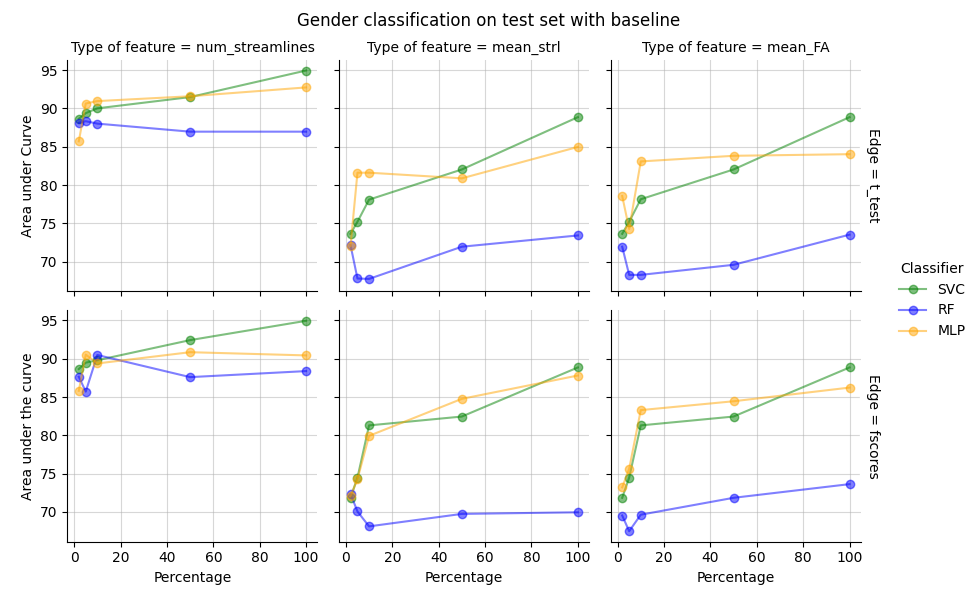
\includegraphics[width=\textwidth]{images/baseline_results_gender.png}
    \caption{Baseline analysis for gender classification. The area under the curve represented as a function of percetange of features. }
    \label{fig:my_label}
\end{figure}
\begin{figure}
    \centering
    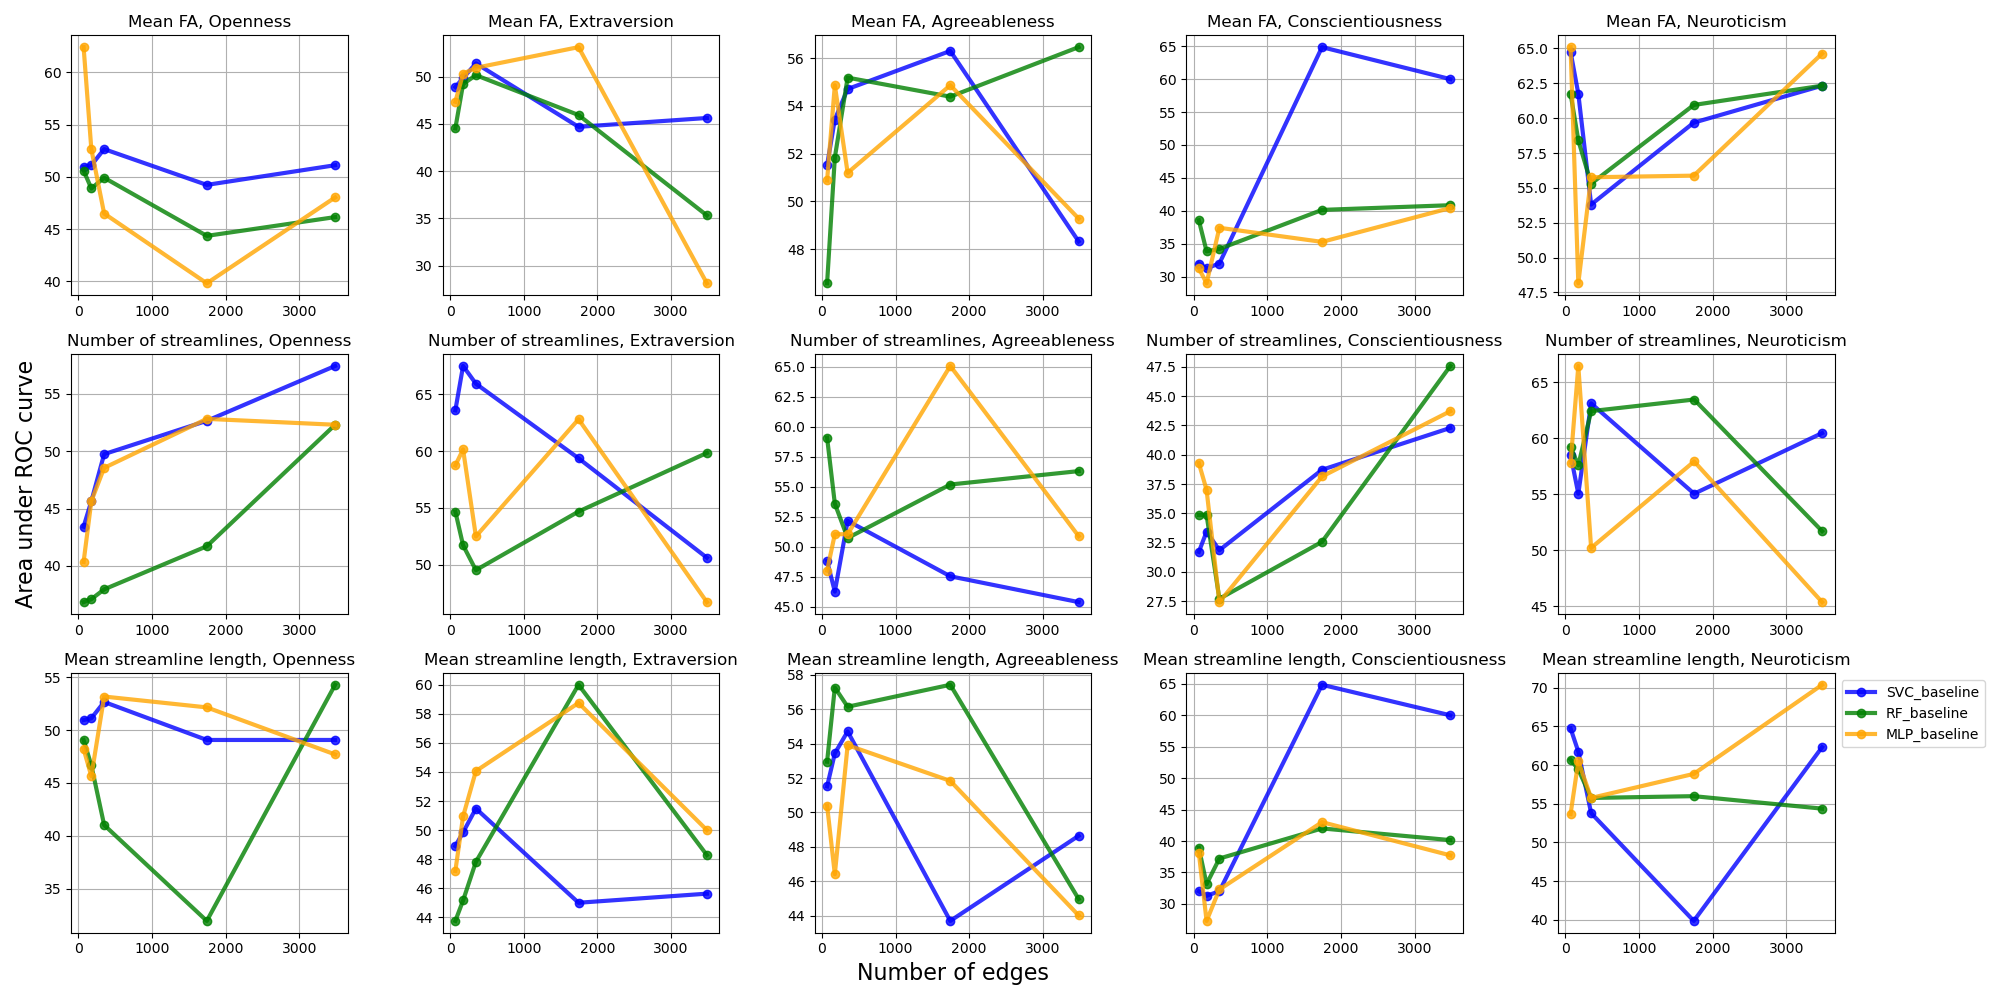
\includegraphics[width=\textwidth]{images/combined_clf_auc_base_personality.png}
    \caption{Baseline analysis on the basis of personality traits. In a general trend it can be seen that doing some feature selection is beneficial for the classification.}
    \label{fig:persona base}
\end{figure}
According to summary.csv,alyze how can we put it
After filtering according to the edges being selected only when there is atleast one streamline per subject. On the basis of the training subjects, the number of features for which all the subjects have a atleast one streamline with them is 1150. The input graph is hence formed on the basis of this with this number determining the upper bound of the number of edges in our input graph. 

\subsection{Output subgraphs}

- they are preserving x edges based on y nodes (specified, our condition was given to be true)
- connected
- subnet scores
- fscores and t-tests are giving similar results
\begin{figure}
    \centering
    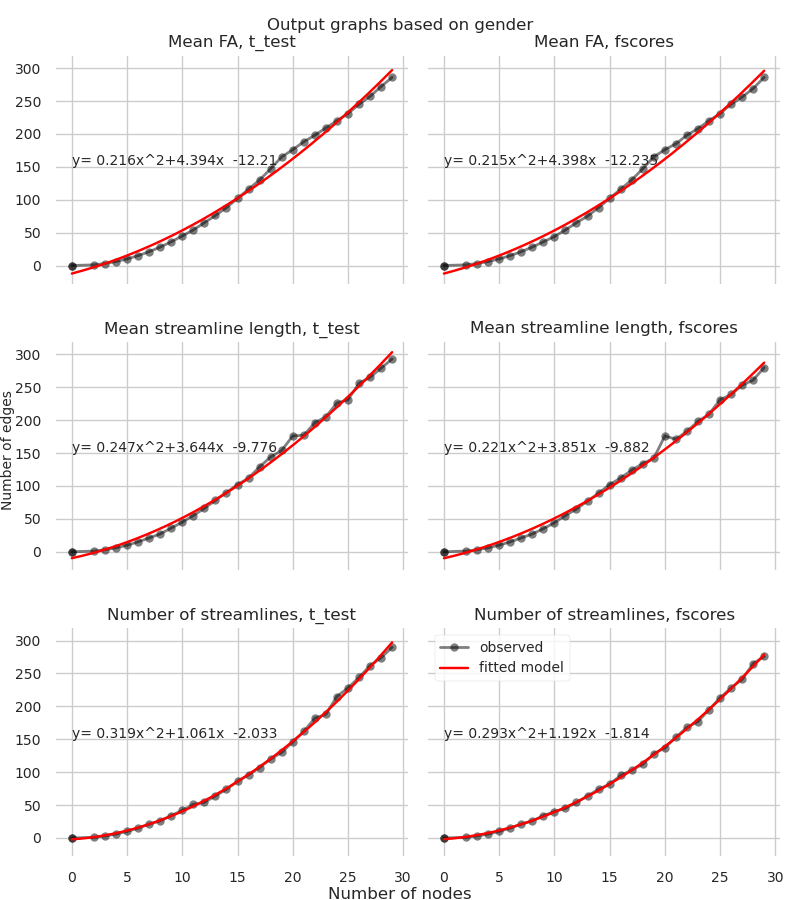
\includegraphics[width=0.8\textwidth]{images/Gender_nodes_preserved.png}
    \caption{Edges preserved as a function of nodes in the case of gender subgraph reduction}
    \label{fig:fun_num_edges}
\end{figure}
\begin{figure}
    \centering
    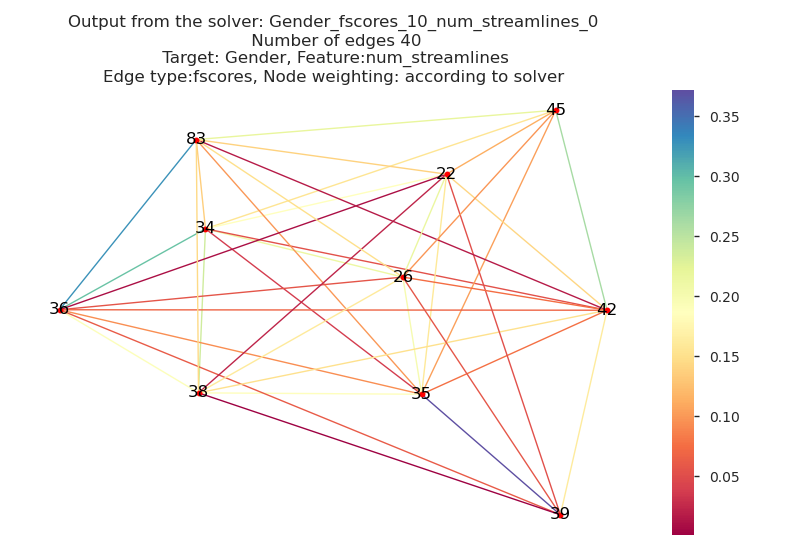
\includegraphics[width=0.5\textwidth]{images/gender10nodes.png}
    \caption{Caption}
    \label{fig:solver_based_gender_10}
\end{figure}


In Fig. \ref{fig:gender_num_strls_10} the MEWS solver based implementation reduces the input graph based on the fscores to infer the most important set of connections. In this graph the edges obtained from Fig. \ref{fig:solver_based_gender_10} were traced back to the original \textit{dataframe} containing the data about number of streamlines for all subjects. The number of streamlines between the regions delineated were determined to put together in the chord graph. From the thickness of the arcs in the chord graph the Left-Palladium and right thalamus proper seem to have the maximum number of connections between them. Further, the subcortical regions seem to have more number of streamlines between them than the cortical regions. 
\begin{figure}
    \centering
    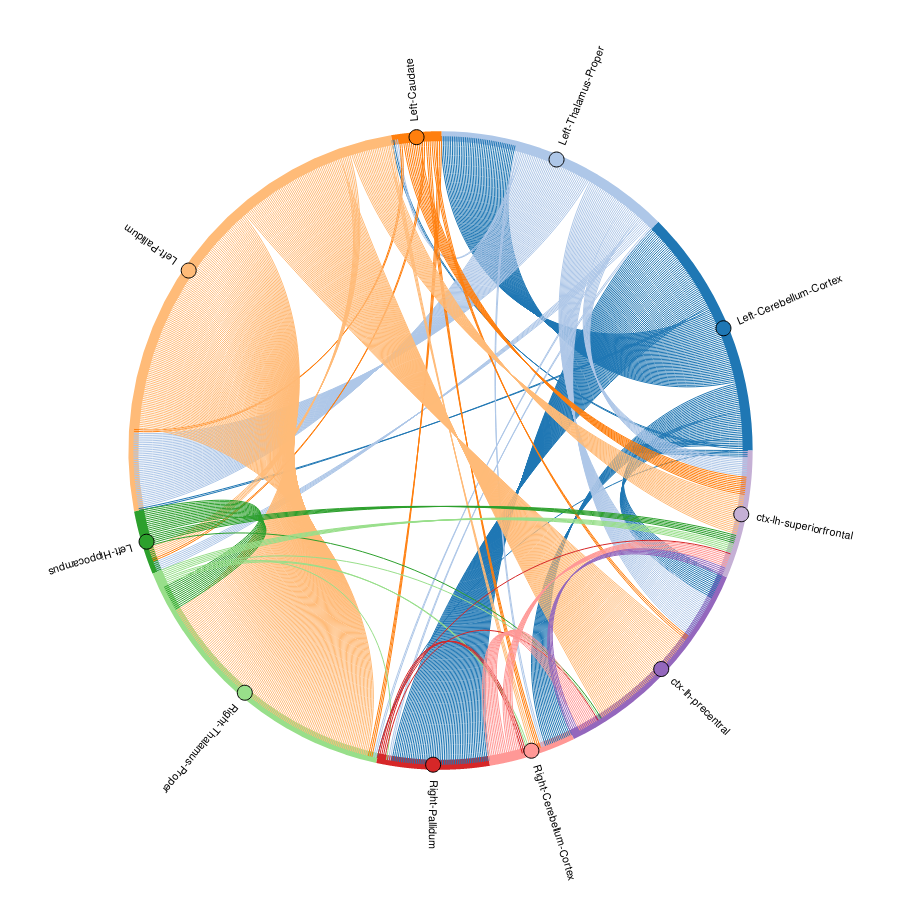
\includegraphics[width=0.9\textwidth]{images/gender10nodes_numstrls.png}
    \caption{10 most important nodes determined using the solver based analysis using the fscores for the Gender based classification. This graph is a Chord graph implemented using Holoviews (\cite{stevens2015holoviews}). The number of edges between any two nodes represent the number of streamlines between them. The fscores were used in order to determine the importance of the connections, the filtered edges retraced back to the original matrix yielded this result. The number of streamlines was averaged for all subjects and then the filtered edges based on the solver were produced. Multiple edges are drawn in the chord type graph where the number of edges represents the number of streamlines.}
    \label{fig:gender_num_strls_10}
\end{figure}


For the features determined by the subgraph. The reduced features were put through an independent samples t-test for gender differences. 
\begin{table}
\label{table:selfloops}
\csvreader[
  tabular=|c*{4}{|c}|,
  table head= \hline feature & ROI & ROI & P value\\ \hline,
  late after last line=\\\hline,
]{tables/gender10_numstrls.csv}{}%
{\csvcoli & \csvcolii & \csvcoliii & \csvcoliv }
\caption{Results for an independent samples t-test carried, The corresponding p values are for the different number of streamlines for males and femalestvod .}
\end{table}


\iffalse
\begin{figure}
    \centering
    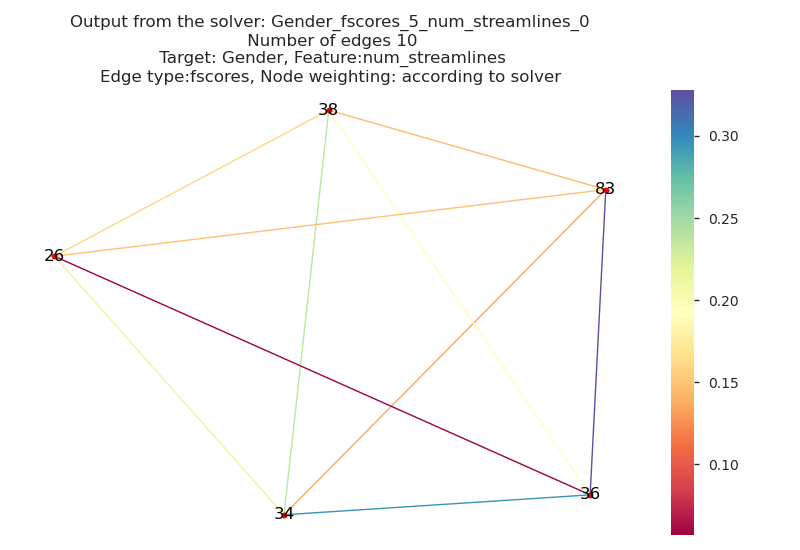
\includegraphics[width=0.8\textwidth]{images/Gender5nodes.png}
    \caption{Caption}
    \label{fig:}
\end{figure}

\begin{figure}
    \centering
    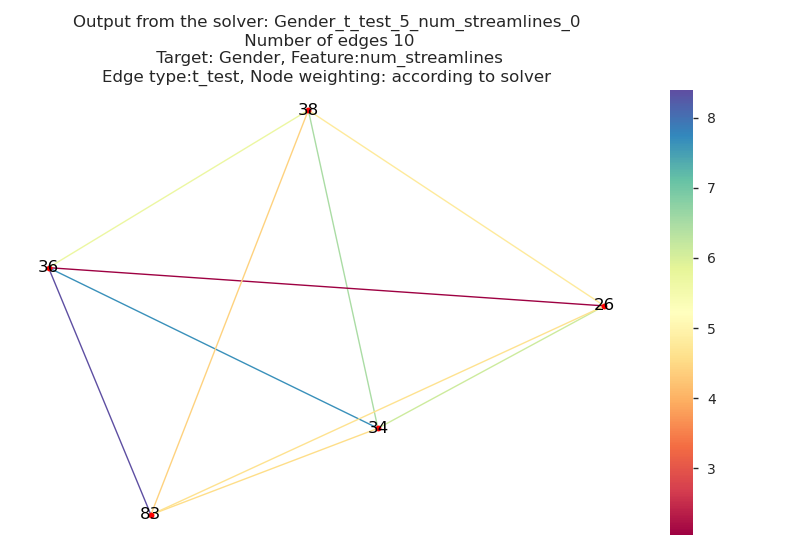
\includegraphics{images/Gender5nodes_test.png}
    \caption{Caption}
    \label{fig:my_label}
\end{figure}
\fi
\iffalse
\section{Solver and baseline comparison}
\begin{figure}
    \centering
    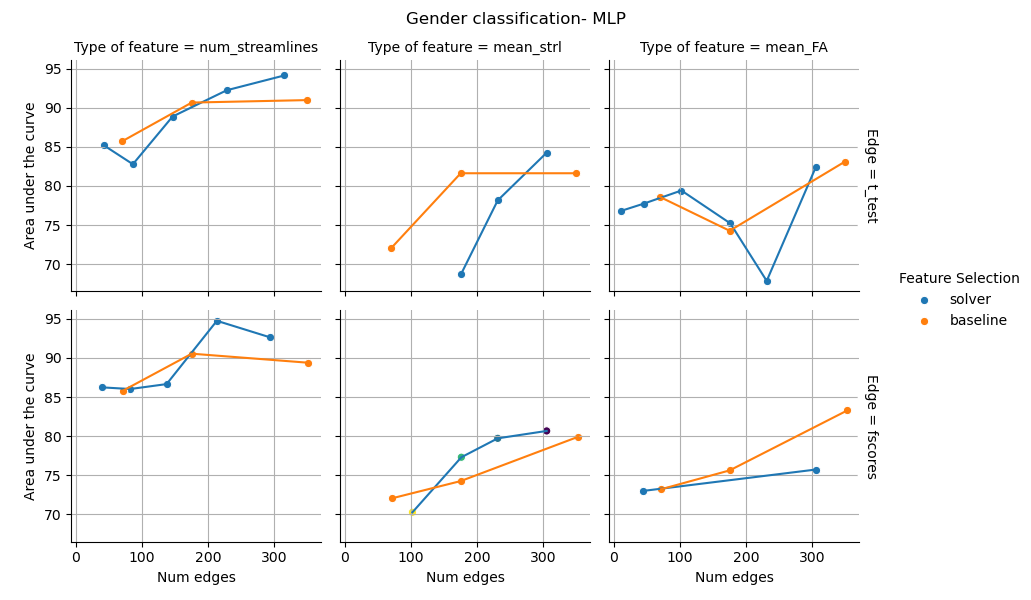
\includegraphics[width = \textwidth]{images/comparison_roc_auc_MLP.png}
    \caption{Caption}
    \label{fig:mlpgender}
\end{figure}
\begin{figure}
    \centering
    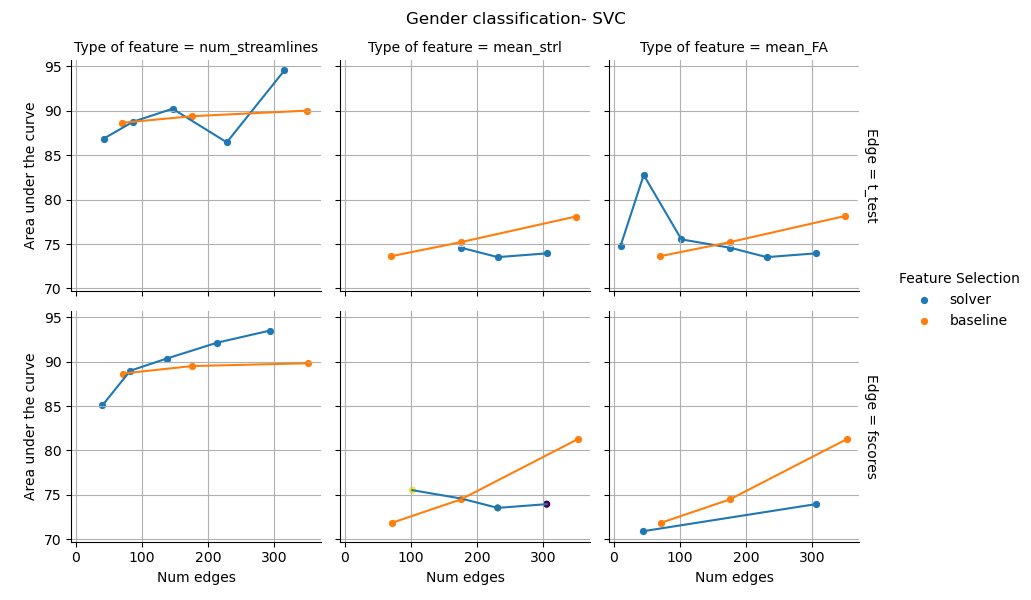
\includegraphics[width = \textwidth]{images/comparison_roc_auc_SVC.png}
    \caption{Caption}
    \label{fig:svcgender}
\end{figure}

\begin{figure}
    \centering
    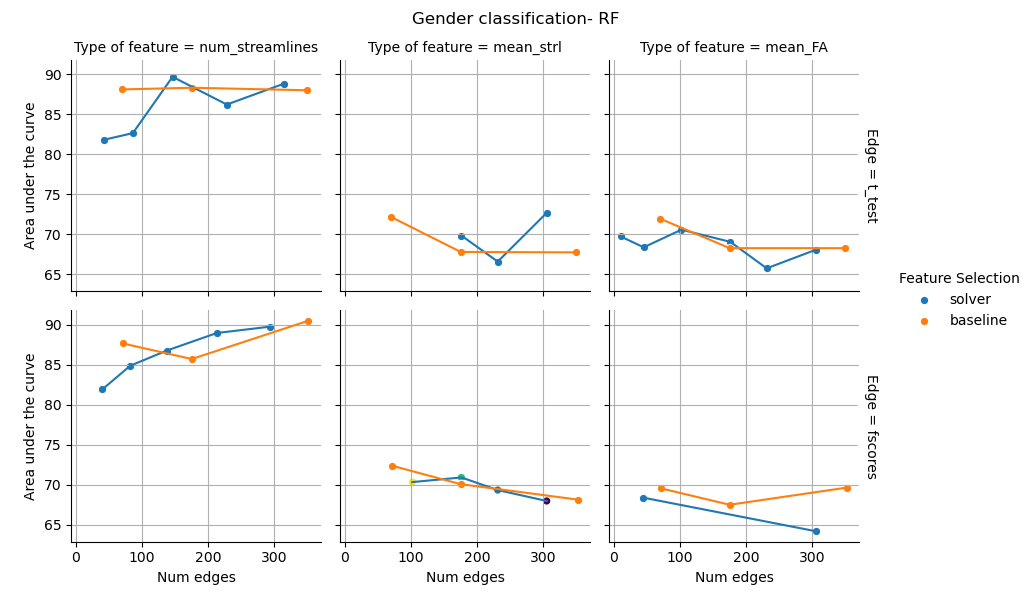
\includegraphics[width = \textwidth]{images/comparison_roc_auc_RF.png}
    \caption{Caption}
    \label{fig:rfgender}
\end{figure}
\fi



\begin{figure}
    \centering
    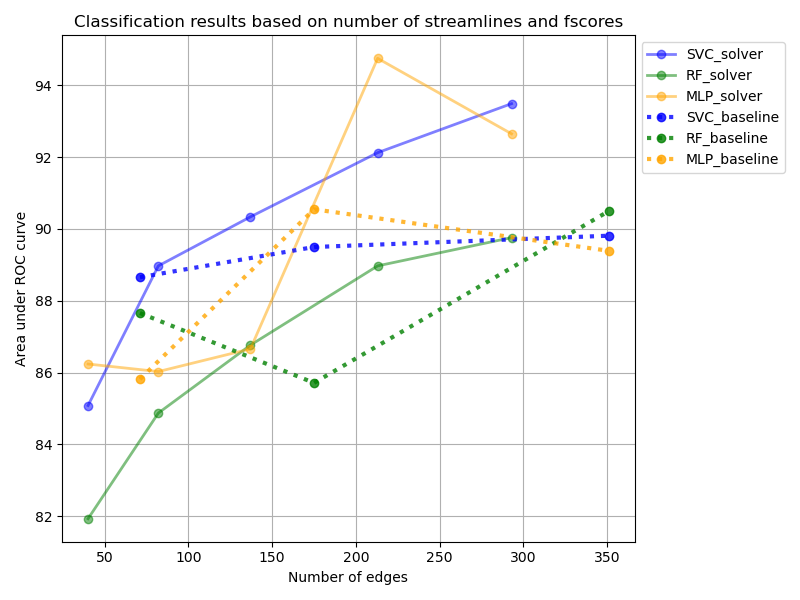
\includegraphics[width=0.8\textwidth]{images/select_clf_auc_gender.png}
    \caption{Comparison of area under the ROC curve for classification on the independent test set. The performance of three classifiers Support Vector Machines, Random Forest and Multilayer perceptron on the basis of features filtered according to the solver and baseline experiments respectively.}
    \label{fig:clf_solver results}
\end{figure}

\iffalse
\begin{figure}
    \centering
    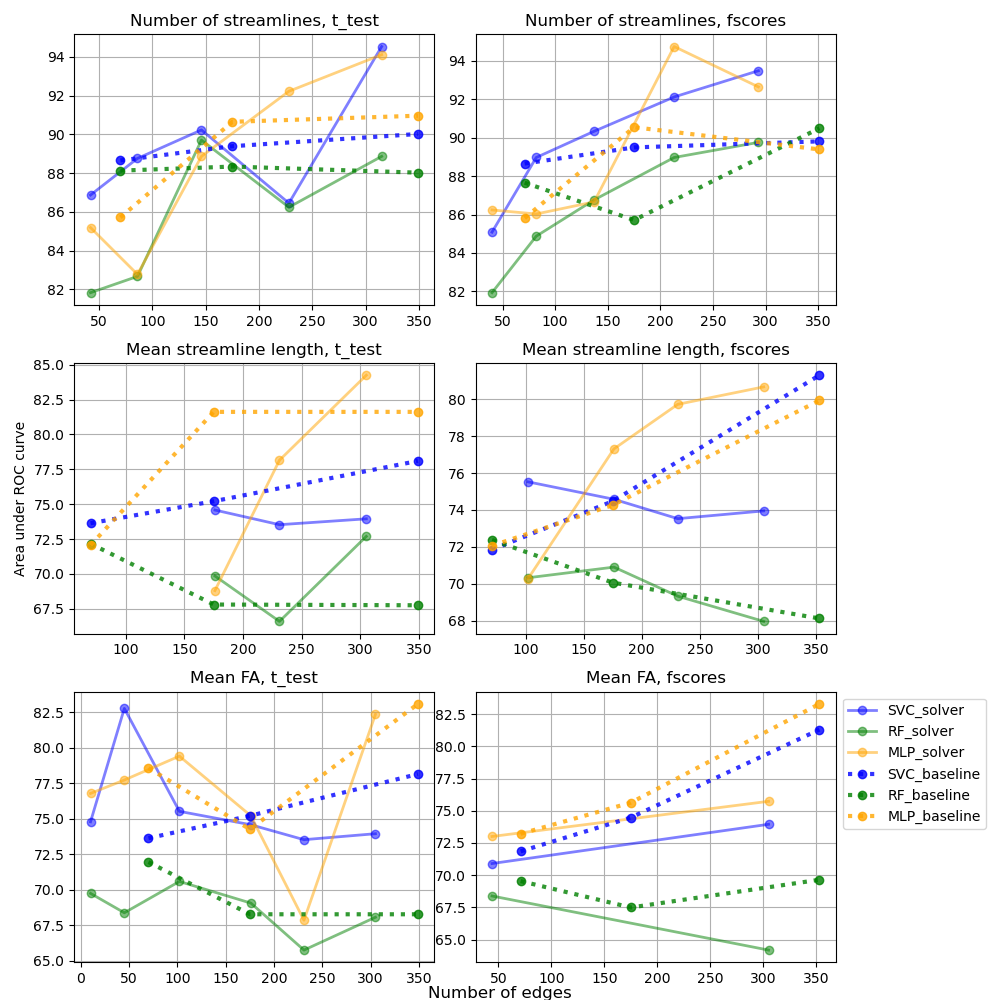
\includegraphics[width=\textwidth]{images/combined_clf_auc_gender.png}
    \caption{ Summary of Gender classification using baseline and solver techniques. In the figure with multiple subplots the rows represent the type of features used and the columns represent the type of edges used for feature ranking with the baseline analysis and as input graph representatives in the solver based approach. The y axis represents the area under the ROC curve for the classification on the test set as a function of the number of edges preserved by either techniques. Each time the number of nodes were specified in terms of percentages for the baseline implementation and as the number of nodes to be preserved for solver based implementation.}
    \label{fig:my_label}
\end{figure}

Judging on the basis of the area under the curve for gender based classification, it is best to compare feature wise.

Consider the mean FA feature first, for this feature the solver based approach does better than or equivalently well as the baseline when the number of edges preserved is small. This is not surprising since the number of edges preserved is a function of the number of nodes specified by the solver based technique. When a specified number of edges would be wanted to be preserved then the features corresponding to only those nodes will be preserved, this makes an inherent bias into which features will be preserved by the solver. Since all one node might have multiple highly relevant performance features but we want to preserve a given number of nodes, so the other less performing feature might be selected since a particular node has to be selected.
\fi


\section{Classification}
\subsection{Best parameters}
For our configuration using Multilayer perceptron for the solver based reduction, classification of gender using the feature selection technique of fscores and refit metric balanced accuracy. Baseline based on 5\% of features.  The parameters for the best estimator of the cross validation turn out to be the same, this justifies that the solver based method works better than the baseline method when it comes to classification accuracy and also leads to an increase in the interpretability.
% Best estimator {'solver': 'adam', 'learning_rate': 'adaptive', 'hidden_layer_sizes': (50, 100, 100, 50), 'alpha': 0.05, 'activation': 'relu'}
% ('MLP', 'Gender', 'random', 'fscores', 'baseline', 'num_streamlines', 5, 'balanced_accuracy', False)
%Bet estimator {'solver': 'adam', 'learning_rate': 'adaptive', 'hidden_layer_sizes': (50, 100, 100, 50), 'alpha': 0.05, 'activation': 'tanh'}
\begin{table}[]
    \centering
    \begin{tabular}{|c|c|c|}
        \hline
        Hyperparameter & Solver & baseline \\
        solver & adam & adam\\
        \hline
        hidden layer size &  50,100,100, 50 & 50,100,100,50\\
        \hline
        activation function & relu & tanh\\
        \hline
        alpha & 0.05 & 0.05\\
        \hline
        learning rate & adaptive & adaptive\\
        \hline
    \end{tabular}
    \caption{Cross validation parameters for MLP trained for gender classification. The parameters which give the best area under the curve for the use case mentioned in the section above have been presented}
    \label{tab:my_label}
\end{table}
\end{document}
